\section{Граничное управление нелинейными волнами деформации в слое двухатомного кристалла}
\begin{frame}[plain, noframenumbering]
    \begin{center}
        \Large
        Граничное управление нелинейными волнами деформации в слое двухатомного кристалла
    \end{center}
\end{frame}

\subsection{Уравнения модели}

\begin{frame}
	\frametitle{Постановка задачи}
Рассматривается изотропный упругий слой,
\begin{itemize}
	\item неограниченной длины в горизонтальном направлении $x$;
	\item шириной $2 H$ в вертикальном направлении $y$;
	\item нижняя поверхность слоя соответствует $y = -H$, верхняя --- $y = H$;
	\item двухатомной структуры.
\end{itemize}   

Вид плотности потенциальной энергии определяется исходя из предположений о двухатомной структуре материала и характере взаимодействия между соседними частицами.

\end{frame}

\begin{frame}
	\begin{center}
		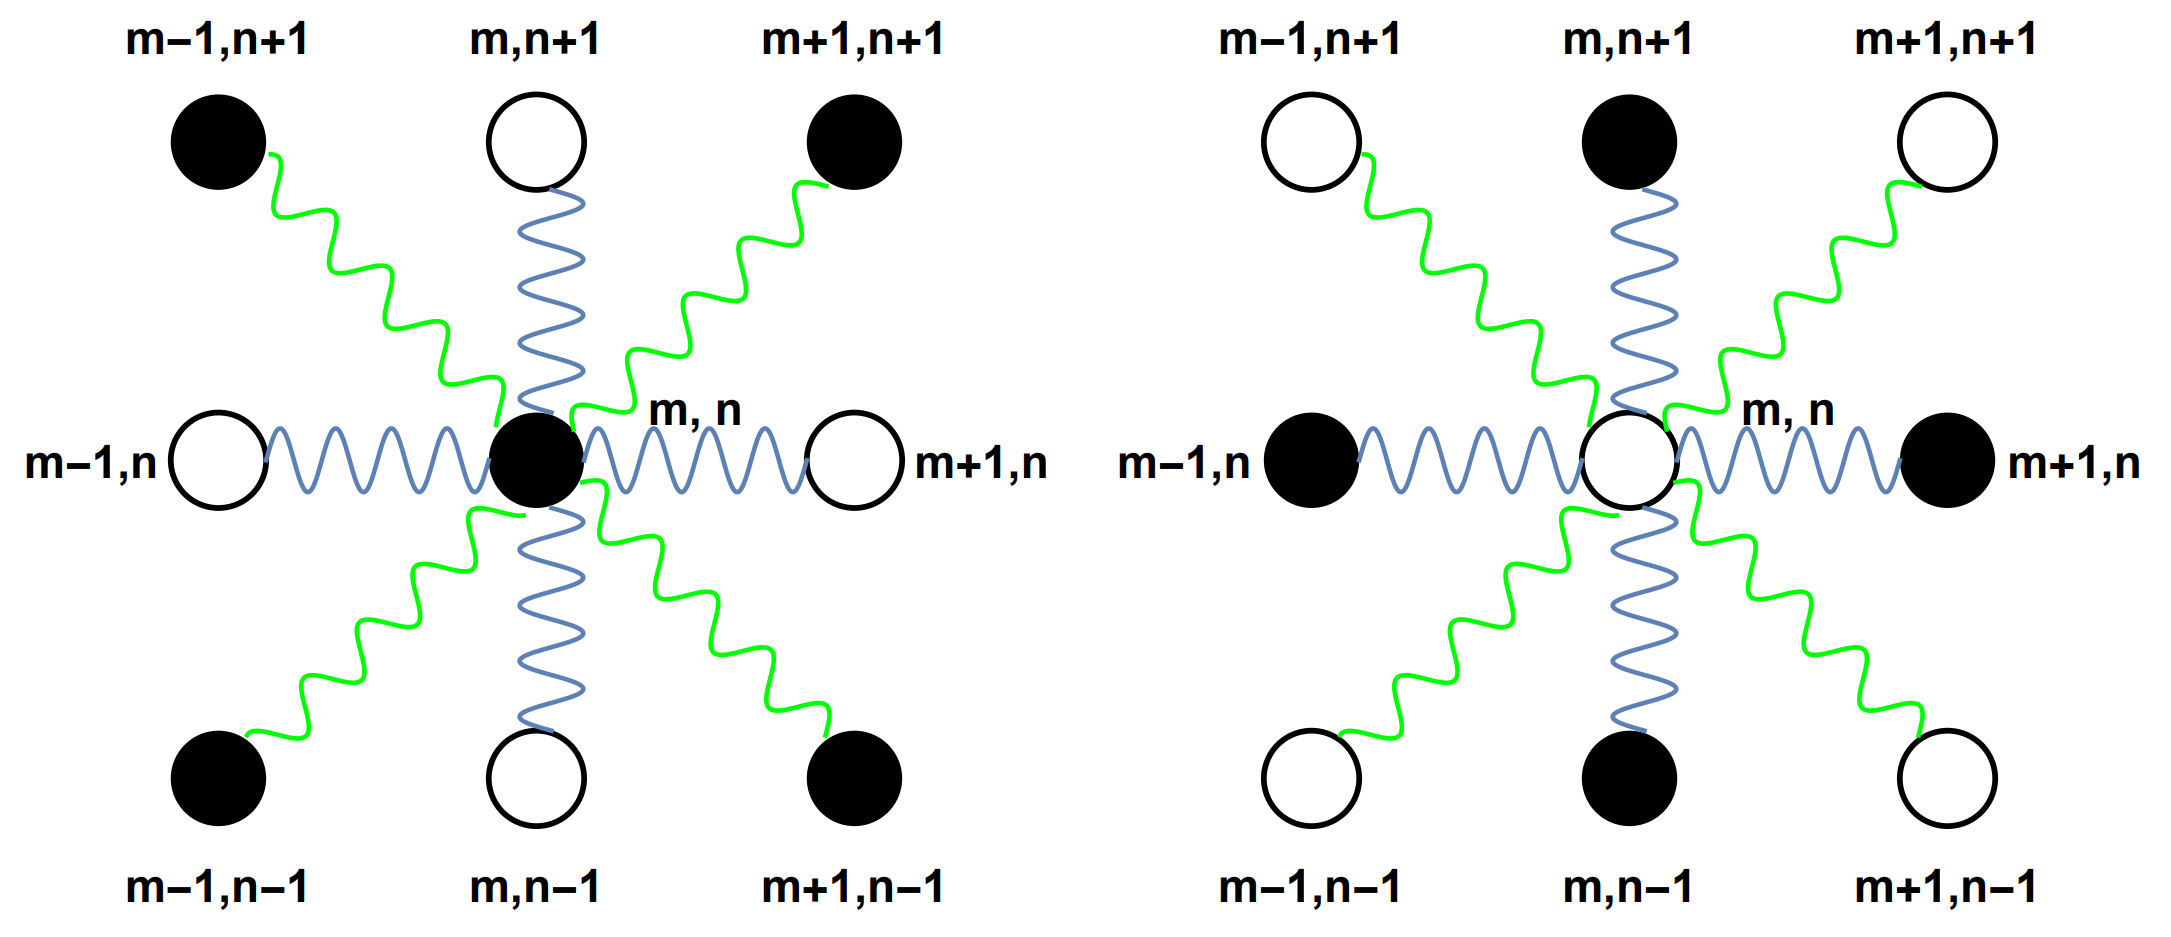
\includegraphics[width=0.85\linewidth]{lattice.png}
	\end{center}
	Система описывается функциями $U$, $u$, $V$, $v$,
	
	$$
	U~=~\frac{m_1~u_1+m_2~u_2}{m_1+m_2},~V=\frac{m_1~v_1+m_2~v_2}{m_1+m_2},
	$$
	$$
	u=\frac{u_1-u_2}{h},~v=\frac{v_1-v_2}{h},
	$$
	где $u_i$, $v_i$ --- горизонтальные и вертикальные смещения элементов двухатомной решетки с массой $m_i$ в континуальном приближении при $h \ll 1$, $i=1,2$ \footnotemark.

\footnotetext[1]{Two-Dimensional Modeling of Diatomic Lattice / A. V. Porubov // Advanced Structured Materials. — Springer International Publishing, 2018. -- С. 263—272.}	
\end{frame}


\begin{frame}
Уравнения движения выводятся с использованием принципа Гамильтона-Остроградского,

$$
\delta \left( \int_{t_0}^{t_1}dt \int_{-H}^{H} dy \int_{-\infty}^{\infty}\left( K - \Pi \right)  \:   dx \right)+ \delta A_1 + \delta A_2=0.
$$

Плотность кинетической энергии равна
$$
	K = \frac{1}{2} \rho (U_t^2 + V_t^2) + \frac{1}{2} \eta (u_t^2 + v_t^2),
$$
\begin{small}
$$
\rho = \frac{m_1+m_2}{h^3}, \quad \eta = \frac{m_1 m_2}{(m_1 + m_2)h}.
$$
\end{small}

Плотность потенциальной энергии условно разделена на две составляющих,
$$
\Pi = \Pi_l + \Pi_{nl}.
$$

\end{frame}


\begin{frame}
	
Линейная часть потенциальной энергии,
\begin{small}
$$
\Pi_l = \frac{C_1}{h} \left(u^2 + v^2\right) + \frac{C_1+C_2}{h}\left(U_x^2+V_y^2\right) +\frac{C_2}{h}\left(U_y^2 + V_x^2 + 2U_x V_y + 2 U_y V_x\right) +
$$
$$
\frac{h\left(C_2\left(m_1^2 + m_2^2\right) - 2C_1 m_1 m_2\right)}{2\left(m_1^2 + m_2^2\right)}\left(u_x^2 + v_y^2\right) + \frac{\left(m_2-m_1\right)\left(C_1+C_2\right)}{m_1+m_2}\left(u_x U_x + v_y V_y\right) +
$$
$$
\frac{C_2 h\left(m_1^2+m_2^2\right)}{2\left(m_1+m_2\right)^2}\left(u_y^2+v_x^2+2u_y v_x + 2u_x v_y\right) +
$$
$$
\frac{C_2\left(m_2 - m_1\right)}{m_1 + m_2}\left(u_y U_y+v_x V_x + u_y V_x + u_x V_y + v_y U_x + v_x U_y\right)
$$
\end{small}

Нелинейная часть потенциальной энергии\footnotemark,
\begin{small}
$$
\Pi_{nl} = \left( p - s_{xx} U_x - s_{yx} \left( U_y + V_x\right) - s_{yy} V_y\right) \left( 1- \cos{(u+v)}\right) \label{pot}
$$
\end{small}		
\footnotetext[2]{The solutions of equations for nonlinear model of deformation of the crystal media allowing martensitic transformations / E. L. Aero, A. N. Bulygin, Y. V. Pavlov // 2017 Days on Diffraction (DD). -- IEEE, 06.2017.
}
\end{frame}

\begin{frame}
\frametitle{Граничные условия}
	
	Выражение для напряжений на границе слоя при $y=-H$ соответствует модели Керра\footnotemark, $q_1$, $q_2$ --- константы, $k_d ~> ~0$ --- коэффициент трения по закону Амонтона-Кулона,
	$$
		\sigma_{y}=q_1 V + q_2 V_t , ~
		\tau_{xy}= k_d (q_1 V + q_2 V_t) \quad | \quad y = -H
	$$
	На верхнюю границу при $y=H$ действует распределенная нагрузка произвольного вида,
	$$
		\sigma_{y}=f_{N}, ~\tau_{xy}=f_{\tau} \quad | \quad y = H
	$$
	
	Соответствующие элементарные работы,
	\begin{small}
	$$
		\delta A_1 =  \int_{t_0}^{t_1} dt\int_{-\infty}^{\infty}f_{N}\delta V \:  dx +\int_{t_0}^{t_1} dt  
		\int_{-\infty}^{\infty} f_{\tau}\delta U \: dx ,
	$$
	$$s
		\delta A_2 =  \int_{t_0}^{t_1} dt \int_{-\infty}^{\infty}(q1_1 V + q_2 V_t)\delta V \:  dx + \int_{t_0}^{t_1} dt
		\int_{-\infty}^{\infty}k_d(q_1 V + q_2 V_t)\delta U \:  dx. 
	$$
	\end{small}

\footnotetext[3]{Elastic and Viscoelastic Foundation Models / A. D. Kerr // Journal of Applied Mechanics. -- 1964. -- Сент. -- Т. 31, № 3. -- С. 491-498.}
\end{frame}

\begin{frame}
\frametitle{Уравнения движения для продольных волн}
\begin{small}	
	Система уравнений движения, полученная из вариационного принципа не приведена в силу громоздкости получаемых выражений и требует применения некоторых упрощений.
	
\begin{itemize}
	\item { Рассматриваются продольные волны, решения в виде степенного ряда по $y$
		\small{
		$$
			U=U_0(x,t)+B_1(x,t)~y+B_2(x,t)~y^2,~u=u_0(x,t)+b_1(x,t)~y+b_2(x,t)~y^2, \label{Usol}
		$$
		$$
			V=y~A(x,t), v=y~a(x,t). \label{Vsol}
		$$
		}
	}
	\item {Упрощается вид нелинейности, предполагается
		$$
		s_{xx} \gg s_{yx}, s_{yy}
		$$
	}
\end{itemize}
	
	Одномерные уравнения для продольных волн относительно $U_0$, полученные в результате процедуры упрощения, имеют вид
\begin{small}
\begin{multline}
	\rho U_{0,tt}-F_1 U_{0,xx}-F_2 u_{0,xx}+F_{31} \left(\cos(u_0)\right)_x = F_5 f_\tau\\
	+ k_d q_1 \left(F_7 U_{0,x}+F_8 u_{0,x}\right)+k_d q_2 \left(F_{11} u_{0,xt}+ F_{13} U_{0,xt}\right),
\end{multline}
\begin{equation}
	\eta u_{0,tt}+f_1 u_0+f_2 u_{0,xx}+f_3 U_{0,xx}+\left(p-s_{xx} U_{0,x}\right)\sin(u_0)=0.  
\end{equation}

\end{small}
\end{small}
\end{frame}

\begin{frame}
	Дальнейшие упрощения связаны с
	\begin{itemize} 
		\item рассмотрением слабонелинейного случая, $u_0 \ll 1$, $U_{0, x} \ll 1$, система приводится к виду
	\begin{multline}
		\rho U_{0,tt}- F_1 U_{0,xx}- F_2 u_{0,xx}-F_{31} u_0 u_{0,x}=F_5 f_\tau\\
		+k_d q_1 (F_7 U_{0,x}+F_8 u_{0,x})+ k_d q_2 (F_{11} u_{0,xt}+ F_{13} U_{0,xt}),
	\end{multline}
	\begin{equation}
		(f_1+p)u_0+f_3 U_{0,xx}-s_{xx} u_0 U_{0,x}=0.
	\end{equation}
		\item рассмотрением длинных волн ($U_{0, xx} \ll U_{0, x}$) и использованием принципа асимптотического подчинения для функции $u$, система сводится к уравнению относительно $U_0$,
		\begin{small}
		\begin{multline}
		\rho U_{0,tt}- F_1 U_{0,xx}+ \frac{f_3 F_2}{f_1+p}U_{0,xxxx}\\+\frac{f_3 s_{xx} F_{2}}{2(f_1+p)^2} (U_{0,x}^2)_{xxx}
		-\frac{f_3^2 F_{31}}{2(f_1+p)^2} (U_{0,xx}^2)_{x}=\\
			F_5 f_\tau+k_d q_1 F_7 U_{0,x} + k_d q_2 F_{11}U _{0,xt}
		\end{multline}
		\end{small}
	\end{itemize}

\end{frame}


\subsection{Алгоритм управления}

\begin{frame}
\frametitle{Алгоритм управления}

Несколько слов о разработанном в предшествующих работах алгоритме управления. В качестве примера рассматривается локализация волновых решений модифицированного уравнения синус-Гордона,
$$
	U_{tt}-U_{xx}+\sin(U)+\omega(x,t)=0,
$$
где $\omega$ --- функция распределенного управления с обратной связью, выражаемая следующим образом,
$$
\omega(x,t)=\gamma \left(\alpha e(x,t)+\alpha_1 e_t(x,t)\right),
$$
$$
e(x,t)=U(x,t)-U^*(x,t),
$$
$$
e_t(x,t)=U_t(x,t)-U^*_t(x,t).
$$
$U^*(x,t)$ --- целевая функция, в качестве которой можно выбрать колоколоообразный солитон, не являющийся точным решением УсГ.
\end{frame}

\begin{frame}
	\begin{figure}
		\begin{center}
			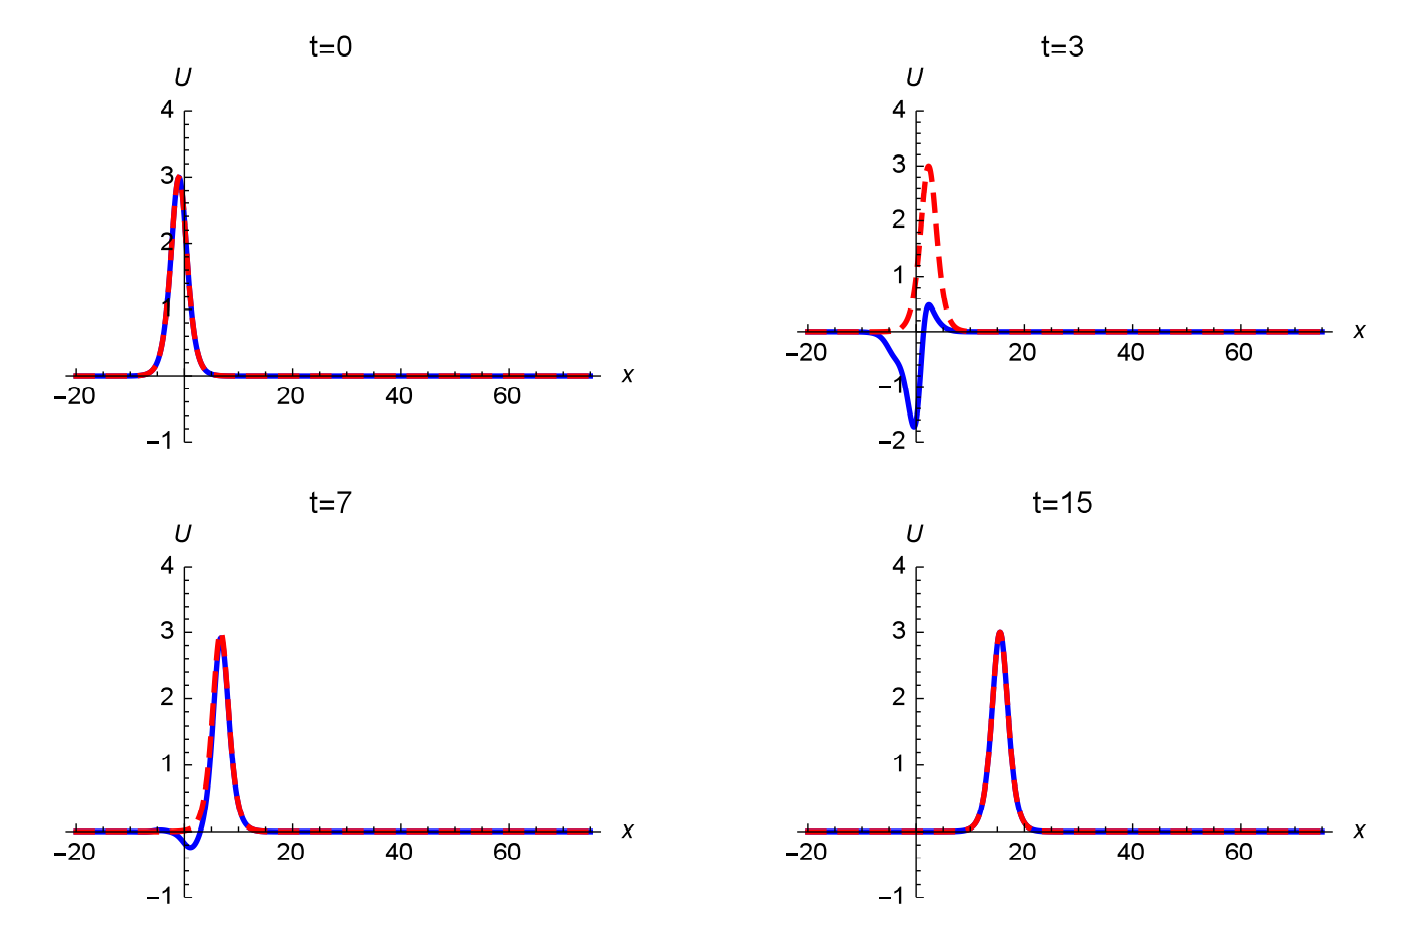
\includegraphics[width=0.9\textwidth]{control_example.png}
		\end{center}
		Пример работы алгоритма, включение при $t = 5$. Синяя линяя --- численное решение, красная пунктирная --- целевая функция вида $A~ {\text{sech}}^2(k (x- t+1))$.
	\end{figure}
\end{frame}

\begin{frame}
	\frametitle{Управление волнами деформации в слое}

Уравнение рассматриваемой системы,
\begin{multline*}
	\rho U_{0,tt}- F_1 U_{0,xx}+ \frac{f_3 F_2}{f_1+p}U_{0,xxxx}\\+\frac{f_3 s_{xx} F_{2}}{2(f_1+p)^2} (U_{0,x}^2)_{xxx}
	-\frac{f_3^2 F_{31}}{2(f_1+p)^2} (U_{0,xx}^2)_{x}=\\
	F_5 f_\tau+k_d q_1 F_7 U_{0,x} + k_d q_2 F_{11}U _{0,xt},
\end{multline*}
в правой части содержит член, который аналогичным образом может играть роль управляющей функции с обратной связью схожего вида,
$$
\omega(x,t)=\gamma \left(\alpha e_x(x,t)+\alpha_1 e_{xt}(x,t)\right),
$$
при выборе внешней нагрузки
$$
f_\tau=-\frac{k_d}{F_5}\left(q_1 F_7 U^*_{0,x}(x,t)+  q_2 F_{11} U_{0,xt}^*(x,t)\right).
$$
\end{frame}	

\subsection{Основные результаты}
\frametitle{Результаты расчетов}
\begin{frame}
	\begin{figure}
		\begin{center}
			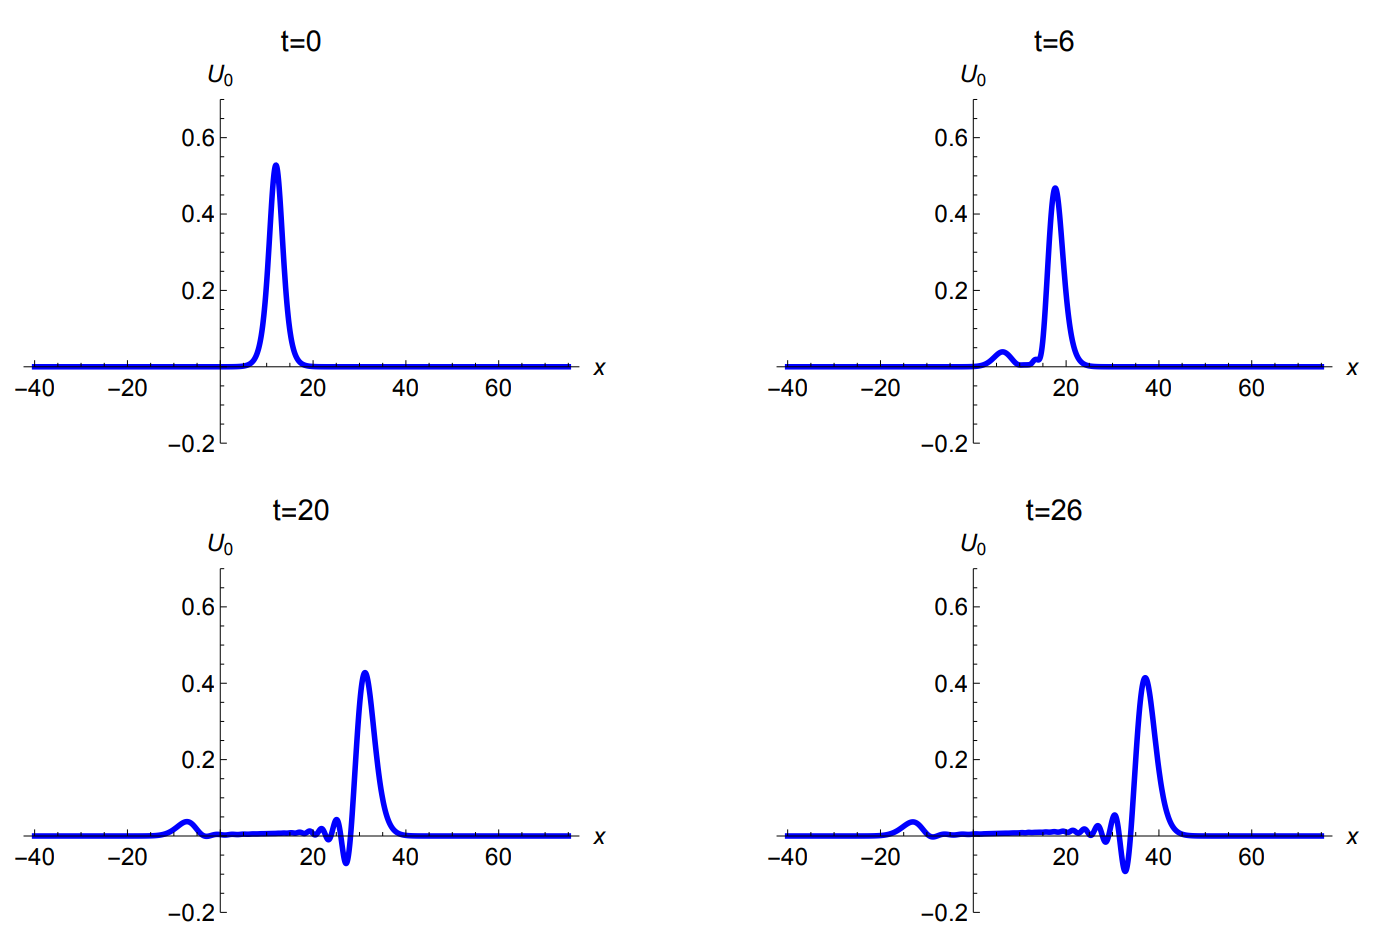
\includegraphics[width=0.9\textwidth]{fig_no_control.png}
		\end{center}
		Распространение колоколообразного начального возмущения вида $A~{\text{sech}}^2 (k (x-V t-x_0))$, внешняя нагрузка $f_\tau$ равна нулю.
	\end{figure}
\end{frame}

\begin{frame}
	\frametitle{Результаты расчетов}
	\begin{figure}
		\begin{center}
			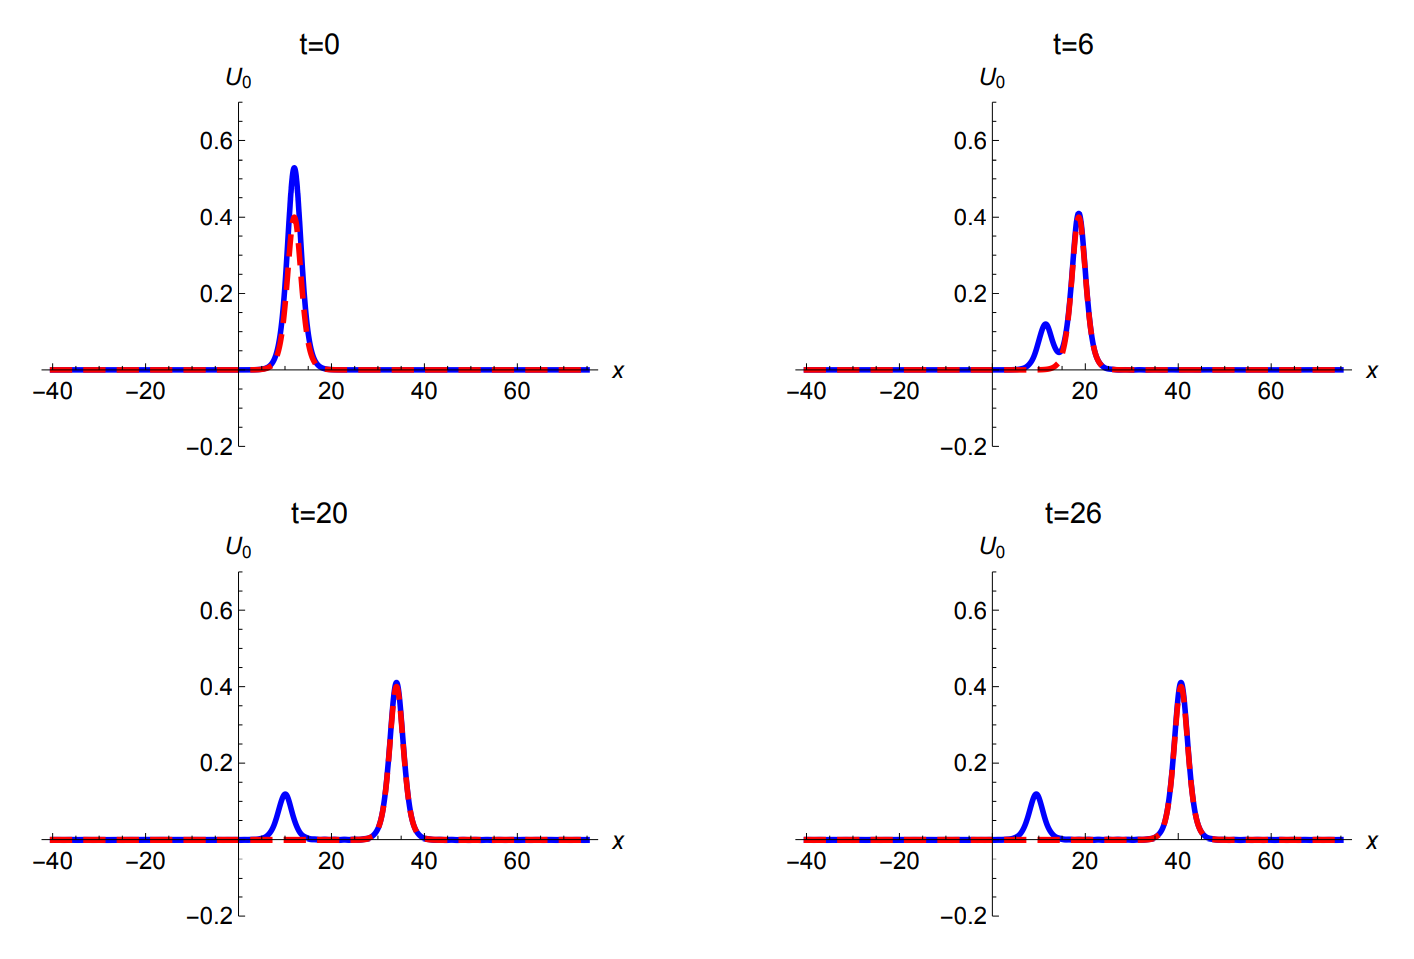
\includegraphics[width=0.9\textwidth]{fig_control.png}
		\end{center}
		Случай с внешней нагрузкой, обеспечивающей наличие управляющей $\omega$ в правой части уравнения. Целевая функция вида $A~{\text{sech}}^2 (k (x-V t-x_0))$.
	\end{figure}
\end{frame}

\begin{frame}
	\frametitle{Результаты}
	Основные результаты данной части работы заключаются в следующем,
	\begin{itemize}
		\item{Получены модельные уравнения, описывающие распространение нелинейных волн деформации в изотропном упругом слое заданной структуры;}
		\item{Показано, что модель допускает наличие распределенного управляющего воздействия с обратной связью, действующего на границе материала;}
		\item{Показано, что выбор нагрузки согласно алгоритму управления, разработанному ранее для схожих механических систем, обеспечивает возможность локализации волн в рассматриваемой системе. }
	\end{itemize}
\end{frame}

\section{Управление гармоническими волнами в акустическом метаматериале}
\begin{frame}[plain, noframenumbering]
	\begin{center}
		\Large
		Управление гармоническими волнами в акустическом метаматериале
	\end{center}
\end{frame}
\subsection{Уравнения модели}

\begin{frame}
	\frametitle{Постановка задачи}
	Рассматривается модель акустического метаматериала <<масса в массе>>, 
	\begin{itemize}
		\item одномерная цепочка, массы $m$ соединены упругими пружинами жесткости $\beta_0 m$;
		\item к каждой частице массы $m$ присоединена масса $m_1$ пружиной линейной жесткости $\beta_1 m_1$, $\eta = m_1/m$;
		\item массы $m_1$ между собой явно не взаимодействуют;
		\item расстояние между соседними частицами --- $h$.
	\end{itemize}   
	
	\begin{center}
		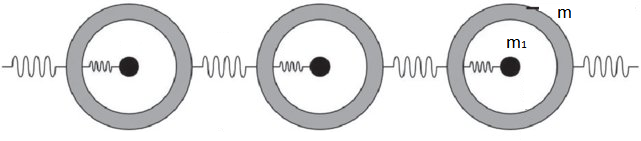
\includegraphics[width=0.7\textwidth]{mim.png}
	\end{center}
	
\end{frame}

\begin{frame}
	Уравнения движения в смещениях $x_n$, $y_n$ для масс $m$, $m_1$ соответственно, выражаются следующим образом,
\begin{equation}
	\ddot{x_n}=\beta_0 (x_{n-1}-2x_n+x_{n+1})+\eta \beta_1 (y_n-x_n), 
	\label{eq1}
\end{equation}
\begin{equation}
	\ddot{y_n}=-\beta_1 (y_n-x_n).
\end{equation}

В континуальном пределе, оставляя первый ненулевой член в ряде Тейлора, уравнения принимают вид
\begin{equation}
	u_{tt}=\beta_0 h^2 u_{xx}+\eta \beta_1 (v-u), \label{eq3}
\end{equation}
\begin{equation}
	v_{tt}=-\beta_1 (v-u). \label{eq4}
\end{equation}
	
\end{frame}

\begin{frame}
	Дисперсионное соотношение системы имеет вид,
	$$
	\omega^4 -(\beta_1(1+\eta)+\beta_0 k^2 h^2)\omega^2+\beta_0 \beta_1 k^2 h^2=0.
	$$
\end{frame}

\subsection{Генерация и управление гармоническими волнами}
\subsection{Основные результаты}
\begin{frame}[plain, noframenumbering]
    \begin{center}
        \Huge
        Графика
    \end{center}
\end{frame}

\begin{frame}
	\frametitle{Результаты расчетов}
\end{frame}

\begin{frame}
    \frametitle{Одиночное изображение}
    \centering
    \includegraphics[width=0.8\linewidth]{latex} % окружение figure не требуется
\end{frame}

\begin{frame}
    \frametitle{Векторная графика}
    \begin{figure}
        \centering
        \ifdefmacro{\tikzsetnextfilename}{\tikzsetnextfilename{tikz_presentation}}{}% присваиваемое предкомпилированному pdf имя файла (не обязательно)
        \input{Presentation/images/tikz_plot.tikz}
    \end{figure}
\end{frame}

%\subsection{Расположение}

\begin{frame}
    \frametitle{Изображения по-вертикали}
    \centering
    \vfill
    \includegraphics[width=0.8\linewidth,height=0.1\textheight]{latex} \\
    \TeX
    \vfill
    \includegraphics[width=0.8\linewidth,height=0.2\textheight]{latex} \\
    \LaTeX
    \vfill
    \includegraphics[scale=0.2]{latex} \\
    \vfill
\end{frame}


\begin{frame}
    \frametitle{Изображения по-горизонтали}
    \begin{minipage}[t]{0.47\linewidth}
        \textbf{Составная \\ подпись 1}
        \center{\includegraphics[width=1\linewidth]{knuth1}}
    \end{minipage}
    \hfill
    \begin{minipage}[t]{0.47\linewidth}
        \textbf{Составная \\ подпись 2}
        \center{\includegraphics[width=1\linewidth]{knuth2}}
    \end{minipage}
\end{frame}

%\subsection{Линии}

\begin{frame}
    \frametitle{Разделяющие линии}
    \begin{minipage}[c]{0.47\linewidth}
        \center{\includegraphics[width=1\linewidth]{latex}}
        \bigskip
        \hrule{}
        \bigskip
        \textbf{Составная \\ подпись 1}
    \end{minipage}
    \hfill
    \vrule{}
    \hfill
    \begin{minipage}[c]{0.47\linewidth}
        \flushright
        \textbf{Составная \\ подпись 2}
        \center{\includegraphics[width=1\linewidth]{knuth2}}
    \end{minipage}
\end{frame}

\section{Численные методы исследования волновых процессов в двумерных решетках}
\subsection{Постановка задачи}
\subsection{Численный метод}
\subsection{Основные результаты}
\begin{frame}[plain, noframenumbering]
    \begin{center}
        \Huge
        Остальное
    \end{center}
\end{frame}

%\subsection{Формулы}

\begin{frame}
    \frametitle{Формулы}
    \[
    \left\{
    \begin{array}{rl}
        \dot x = & \sigma (y-x)  \\
        \dot y = & x (r - z) - y \\
        \dot z = & xy - bz
    \end{array}
    \right.
    \]
\end{frame}

\begin{frame}
    \frametitle{amsmath}
    \centering
    \begin{minipage}[t]{0.5\linewidth}
        \begin{multline*}
            y = 1 x^1 + 2 x^2 + 3 x^3 + \\ + 4 x^4 + 5 x^5 + \dots
        \end{multline*}
    \end{minipage}
\end{frame}

\begin{frame}[allowframebreaks]
    \frametitle{Уравнения Максвелла}
    \centering{
        \small
        \def\arraystretch{1.8}%
        \begin{tabular}{ll}
            \toprule
            Интегральная форма                                                                                                                                            & Дифференциальная форма                                                          \\ \midrule
            \(Q_e(t) = \displaystyle\oiint_S \vec D(t) \cdot d\vec{s} = \displaystyle\iiint_V \rho_v(t) dv\)                                                              & \(\nabla \cdot \vec D(t) = \rho_v(t)\)                                          \\
            \(\displaystyle\oiint_S \vec B(t) \cdot d\vec{s} = 0\)                                                                                                        & \(\nabla \cdot \vec B(t) = 0\)                                                  \\
            \(V_{emf}(t) = \displaystyle\oint_L \vec E(t) \cdot d\vec{l}\) = \(- \displaystyle\iint_S \left[\frac{\partial\vec{B}(t)}{\partial t}\right] \cdot d\vec{s}\) & \(\nabla \times \vec E(t) = - \frac{\partial\vec{B}(t)}{\partial t}\)           \\
            \(I(t) = \displaystyle\oint_L \vec H(t) \cdot d\vec{l} = \displaystyle\iint_S \left[\vec J(t) + \frac{\partial\vec{D}(t)}{\partial t}\right] \cdot d\vec{s}\) & \(\nabla \times \vec H(t) = \vec J(t) + \frac{\partial\vec{D}(t)}{\partial t}\) \\ \midrule
            \(\displaystyle\oiint_S \vec J \cdot d\vec{s} = -\frac{\partial Q_e}{\partial t}\)                                                                            & \(\nabla \cdot \vec J = - \frac{\partial \rho_v}{\partial t}\)                  \\
            \bottomrule
            \multicolumn{2}{c}{\(\vec D(t) = \left[\varepsilon(t)\right] * \vec E(t)\)}                                                                                                                                                                     \\
            \multicolumn{2}{c}{\(\vec B(t) = \left[\mu(t)\right] * \vec H(t)\)}                                                                                                                                                                             \\
        \end{tabular}
    }
    \framebreak

    \hspace{0.05\linewidth}
    \centering{
        \small
        \def\arraystretch{1.8}%
        \begin{tabular}{ll}
            \toprule
            Интегральная форма                                                                                                                & Дифференциальная форма                               \\ \midrule
            \(Q_e = \displaystyle\oiint_S \vec D \cdot d\vec{s} = \displaystyle\iiint_V \rho_v dv\)                                           & \(\nabla \cdot \vec D = \rho_v\)                     \\
            \(\displaystyle\oiint_S \vec B \cdot d\vec{s} = 0\)                                                                               & \(\nabla \cdot \vec B = 0\)                          \\
            \(V_{emf} = \displaystyle\oint_L \vec E \cdot d\vec{l}\) = \(- \displaystyle\iint_S \left[j \omega \vec B\right] \cdot d\vec{s}\) & \(\nabla \times \vec E = - j \omega \vec B\)         \\
            \(I = \displaystyle\oint_L \vec H \cdot d\vec{l} = \displaystyle\iint_S \left[\vec J + j \omega \vec D\right] \cdot d\vec{s}\)    & \(\nabla \times \vec H = \vec J + j \omega \vec{D}\) \\ \midrule
            \(\displaystyle\oiint_S \vec J \cdot d\vec{s} = - j \omega Q_e\)                                                                  & \(\nabla \cdot \vec J = - j \omega \rho_v\)          \\
            \bottomrule
            \multicolumn{2}{c}{\(\vec D(t) = \left[\varepsilon\right] \vec E(t)\)}                                                                                                                   \\
            \multicolumn{2}{c}{\(\vec B(t) = \left[\mu\right] \vec H(t)\)}                                                                                                                           \\
        \end{tabular}
    }
\end{frame}

%\subsection{Таблицы}

\begin{frame}
    \frametitle{Таблица}
    \centering
    \begin{tabular}{|l|l|}
        \hline
        \textbf{Заголовок 1} & \textbf{Заголовок 2} \\
        \hline
        Сумма                & \(b+a\)              \\
        \hline
        Разность             & \(a-b\)              \\
        \hline
        Произведение         & \(a*b\)              \\
        \hline
    \end{tabular}
\end{frame}

\begin{frame}
    \frametitle{Другая таблица}
    \centering
    \begin{tabular}{lc}
        \toprule
        \multicolumn{1}{c}{\textbf{Заголовок 1}} & \textbf{Заголовок 2} \\ \midrule
        Сумма                                    & \(b+a\)              \\
        Разность                                 & \(a-b\)              \\
        Произведение                             & \(a*b\)              \\
        \bottomrule
    \end{tabular}
\end{frame}


%\subsection{Разное}

\begin{frame}
    \frametitle{Большой многоуровневый список}
    \begin{itemize}
        \item \textbf{Пункт 1}
              \begin{itemize}
                  \itemi Подпункт 1-1
                  \itemi Подпункт 1-2
              \end{itemize}
        \item \textbf{Пункт 2}
              \begin{itemize}
                  \itemi Подпункт 2-1
              \end{itemize}
        \item \textbf{Пункт 3}
              \begin{itemize}
                  \itemi Подпункт 3-1
                  \itemi Подпункт 3-2
              \end{itemize}
        \item \textbf{Пункт 4}
              \begin{itemize}
                  \itemi Подпункт 4-1
              \end{itemize}
        \item \textbf{Пункт 5}
              \begin{itemize}
                  \itemi Подпункт 5-1
                  \itemi Подпункт 5-2
                  \itemi Подпункт 5-3
              \end{itemize}
    \end{itemize}
\end{frame}

\begin{frame}
    \frametitle{Четыре изображения}
    \centering
    \includegraphics[width=0.35\linewidth,angle=35]{latex}
    \includegraphics[width=0.35\linewidth,angle=135]{latex}\\
    \includegraphics[width=0.35\linewidth,angle=15]{latex}
    \includegraphics[width=0.35\linewidth,angle=-15]{latex}
\end{frame}

